\chapter{Lezione 8}
\label{chap:lezione_08} 

\begin{flushright}
\textit{Data: 20/10/2025}
\end{flushright}

\section{Soluzioni in MFA con Campo Magnetico Nullo}

L'obiettivo è comprendere il comportamento della magnetizzazione $m$, in funzione di parametri come la temperatura $T$ (o $\beta$) e il campo magnetico $h$. L'approccio adottato è quello della \textbf{Teoria di Campo Medio} (MFA). Questa approssimazione si basa sull'assunzione che gli spin siano \textbf{scorrelati}.

\noindent Iniziamo analizzando la situazione in campo magnetico nullo, $h=0$. 

L'equazione per la magnetizzazione si deriva da:
\begin{equation}
f'(m)=-2Dm+\frac{1}{2\beta}\log\frac{1+m}{1-m} = 0
\end{equation}
dove $D$ è una costante che dipende dalla geometria del reticolo.

Questa è la stessa equazione trovata in precedenza, che ha soluzioni non banali solo per valori bassi della pendenza (ovvero solo per basse temperature). Ricordiamo che la soluzione $m=0$ è sempre una soluzione.

\vspace{0.5cm}

Per determinare la stabilità delle soluzioni, si deve analizzare la derivata seconda $f''(m)$. Una soluzione è un minimo di $f(m)$ se $f''(m) > 0$. 

\noindent La \textbf{temperatura critica} è: $T_c=2D$      ( $\beta_c = \frac{1}{2D}$)

\subsubsection{Caso $T > T_c$ (Alta Temperatura)}

Quando la temperatura è maggiore della temperatura critica ($T > T_c$), ovvero $\beta < \beta_c$, si ha la condizione $2D\beta < 1$.
In questo regime:
\begin{itemize}
    \item La derivata seconda è maggiore di zero ($f''(m) > 0$) per tutti i valori di $m$ nell'intervallo fisicamente rilevante $(-1, 1)$
    \item C'è \textbf{un solo minimo} globale in $m=0$
    \item L'energia libera $f(m)$ ha un comportamento di tipo parabolico (armonico) attorno a $m=0$
    \item C'è solo una soluzione all'equazione del campo medio.
\end{itemize}

\subsubsection{Caso $T < T_c$ (Bassa Temperatura)}

Quando la temperatura è minore della temperatura critica ($T < T_c$), ovvero $2D\beta > 1$ , si è nel regime di \textbf{fase fredda} o \textbf{fase a simmetria rotta} (cold / broken phase).
\begin{itemize}
    \item La derivata seconda  calcolata in $m=0$ è negativa: $f''(m=0) < 0$
    
    La soluzione $m=0$ non è più un minimo, ma un \textbf{massimo}.
    \item Esistono \textbf{due minimi locali} in $m = + \tilde{m} = m^{+}$ e $m = - \tilde{m} = m^{-}$
    
    Questi due minimi devono essere opposti per ragioni di simmetria.
   
\end{itemize}


\subsubsection{Caso $T = T_c$ (Punto Critico)}

Al punto critico $T = T_c$ ($\beta = \beta_c$), si ha $2D\beta = 1$.
\begin{itemize}
    \item La curva $f(m)$ si \textbf{appiattisce} in $m=0$
    \item Si ha $f''(m=0)=0$
\end{itemize}

\vspace{0.5cm}

\begin{figure}[h!]
    \centering
    \begin{minipage}[b]{0.4\textwidth}
        \centering
        \includegraphics[width=\textwidth]{pics/03.png}
    \end{minipage}
    \hfill
    \begin{minipage}[b]{0.4\textwidth}
        \centering
        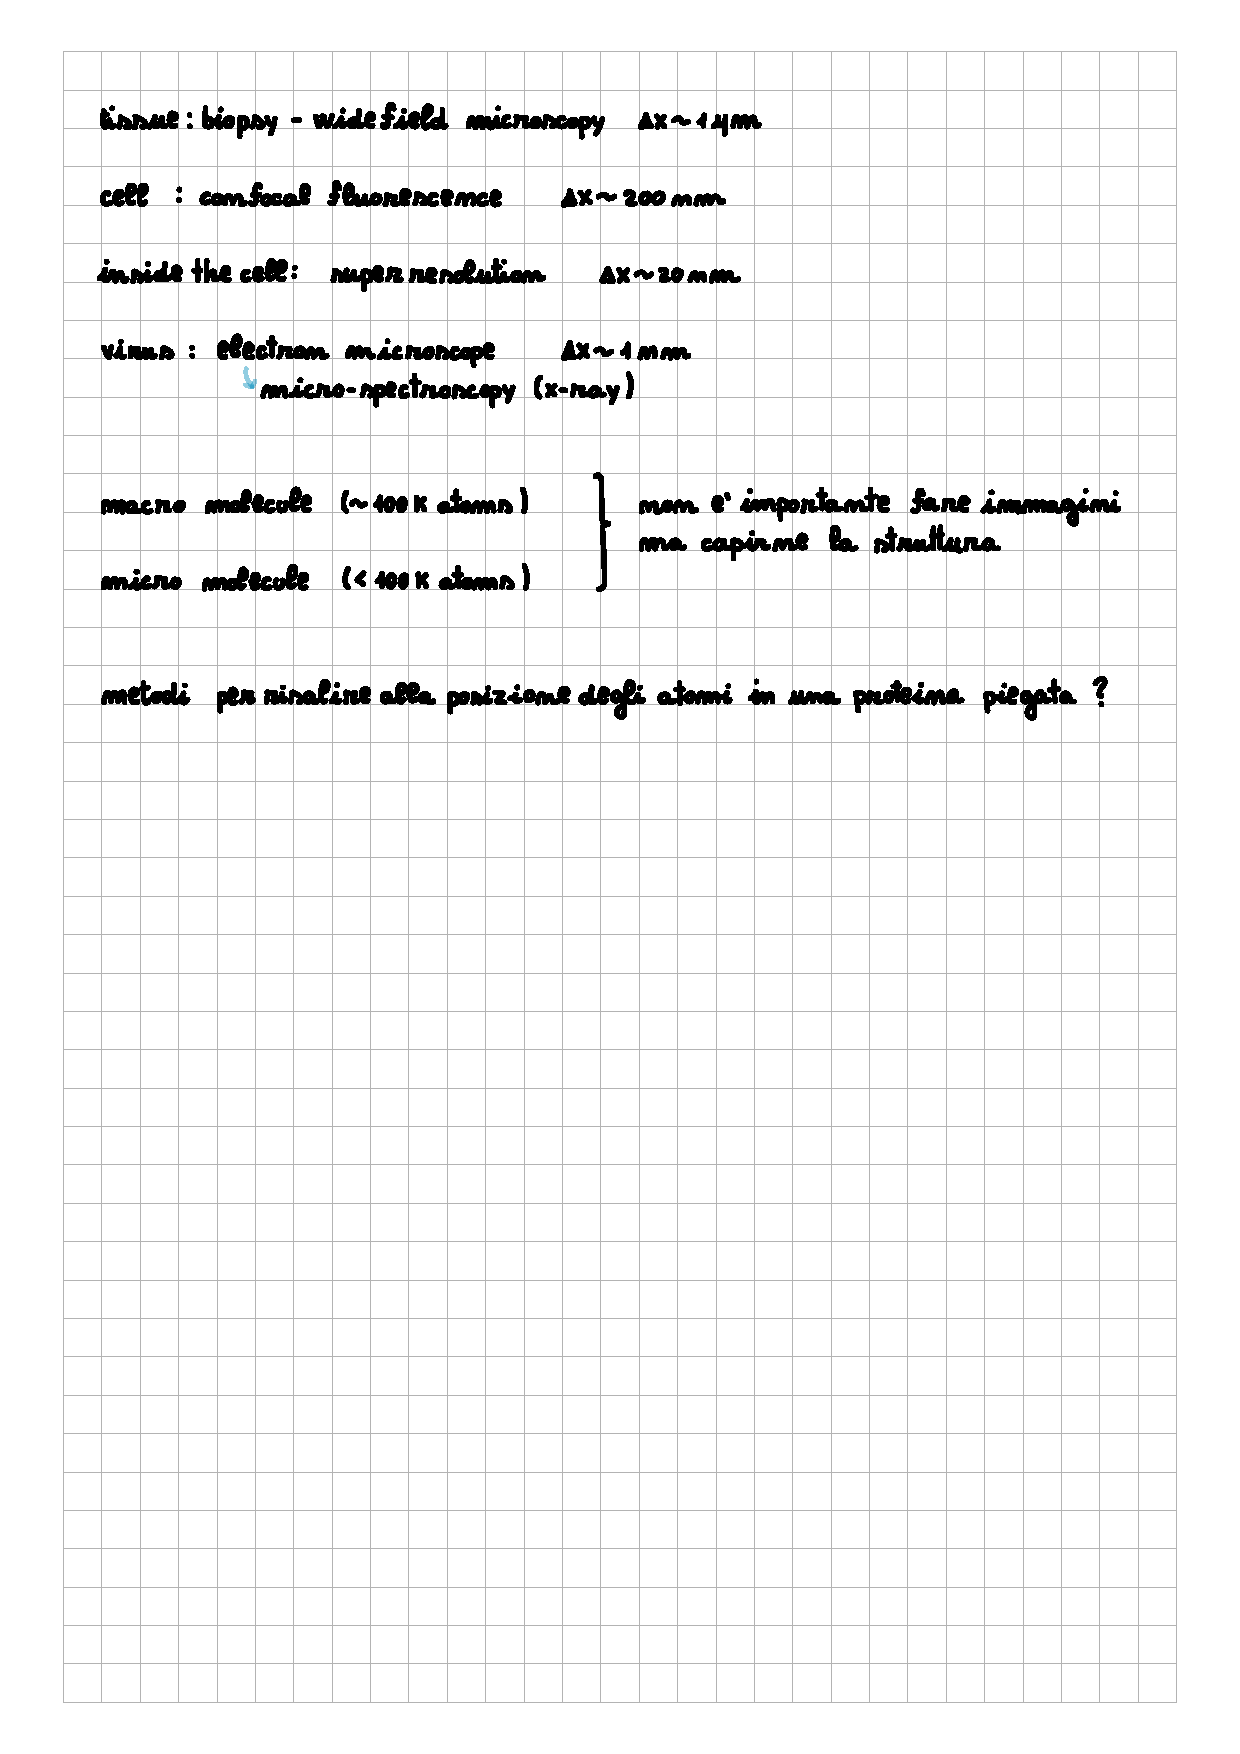
\includegraphics[width=\textwidth]{pics/04.png}
    \end{minipage}

    \begin{minipage}[b]{0.5\textwidth}
        \centering
        \includegraphics[width=\textwidth]{pics/05.png}
    \end{minipage}
    \caption{Andamento di $f(m)$ al variare della temperatura.}
    \label{fig:8.1}
\end{figure}

Se il sistema venisse preparato in uno stato random ($m \approx 0$) a $T < T_c$, esso evolverebbe spontaneamente (cadrebbe) verso uno dei due minimi stabili, $m^{+}$ o $m^{-}$, acquisendo una magnetizzazione spontanea.

\newpage
\subsection{Espansione vicino al Punto Critico}

Vicinissimo al punto critico, per $T \to T_c^-$ , si ha $m \to 0$

La magnetizzazione spontanea è piccola e si procede espandendo l'equazione del campo medio in potenze di $m$. L'equazione di partenza è:
\begin{equation}
f'(m)=-2Dm+\frac{1}{2\beta}\log\frac{1+m}{1-m} = 0
\end{equation}

Si utilizza l'\textbf{espansione in serie di Taylor} per $\log(\frac{1+m}{1-m})$ intorno a $m=0$. Per ricavarla, si parte dalle espansioni di $(1-m)^{-1}$ e $\log(1+x)$.

\begin{itemize}
    \item Espansione di $(1-m)^{-1}$:
    \begin{equation*}
    (1-m)^{-1} \approx 1+m+m^{2}+m^{3}+O(m^{4}) 
    \end{equation*}
    \item Espansione di $\frac{1+m}{1-m}$:
    \begin{align*}
        \frac{1+m}{1-m} &\approx (1+m)(1+m+m^{2}+m^{3})+O(m^{4})\\ &= 1+2m+2m^{2}+2m^{3}+O(m^{4})
    \end{align*}
    \item Sostituendo nel logaritmo:
    \begin{equation*}
    \log\frac{1+m}{1-m} \approx \log( 1 + 2 (m+m^{2}+m^{3}))
    \end{equation*}
    \item Espansione di $\log(1+x)$:
    \begin{equation*}
    \log(1+x) \approx x-\frac{x^{2}}{2}+\frac{x^{3}}{3}+O(x^{4})
    \end{equation*}
    \item Ponendo $x = 2m+2m^2+2m^3 $ :
    \begin{equation*}
    \log\frac{1+m}{1-m} \approx 2(m+m^{2}+m^{3})-\frac{4}{2}(m+m^{2})^{2}+\frac{8}{3}m^{3}+O(m^{5})
    \end{equation*}
\end{itemize} 

Raccogliendo i termini dello stesso ordine in $m$, l'espansione è:
\begin{equation}
\log\frac{1+m}{1-m} \approx 2m + \frac{2}{3}m^3 + O(m^4)
\end{equation}

Sostituendo nell'equazione del campo medio:
\begin{tcolorbox}[colback=yellow!30,  
                  colframe=yellow!50!orange,  
                  boxrule=0.8pt, 
                  arc=3pt,  
                  top=4pt, bottom=4pt, left=6pt, right=6pt,
                  enhanced,
                  sharp corners=south]
\begin{equation}
f'(m) = -2Dm+\frac{1}{2\beta}\left(2m+\frac{2}{3}m^3\right)  \quad \quad \quad \text{  per  }\; T \to T_c^- \; , \; m \to 0
\end{equation}
\end{tcolorbox} 

Questa equazione ha la soluzione banale $m=0$. Cerchiamo le soluzioni non nulle ($m \ne 0$) che esistono per $T < T_c$:
\begin{equation}
-2D + \frac{1}{\beta} + \frac{m^2}{3\beta} = 0
\end{equation}
Risolviamo per $m^2$:
\begin{equation}
\frac{m^2}{3\beta} = 2D - \frac{1}{\beta} = \frac{2D\beta - 1}{\beta}
\end{equation}
\begin{equation}
m^2 = 3\beta \left( \frac{2D\beta - 1}{\beta} \right) = 3(2D\beta - 1)
\end{equation}
Quindi la magnetizzazione spontanea $m$ è:
\begin{tcolorbox}[colback=yellow!30,  
                  colframe=yellow!50!orange,  
                  boxrule=0.8pt, 
                  arc=3pt,  
                  top=4pt, bottom=4pt, left=6pt, right=6pt,
                  enhanced,
                  sharp corners=south]
\begin{equation}
m = \pm \sqrt{3}(2D\beta-1)^{\frac{1}{2}} \quad \quad \quad \text{  per  }\; T \to T_c^- \; , \; m \to 0
\end{equation}
\end{tcolorbox} 

Questo risultato definisce il primo \textbf{esponente critico} che incontriamo, chiamato $\beta$ (da non confondere con $1/k_B T$). 

La magnetizzazione $m$ vicino alla temperatura critica $T_c$ (dal basso) segue la legge:

\begin{equation}
m \propto (\beta - \beta_c)^{1/2} \propto (T_c - T)^{1/2}
\end{equation}

\begin{tcolorbox}[colback=yellow!30,  
                  colframe=yellow!50!orange,  
                  boxrule=0.8pt, 
                  arc=3pt,  
                  top=4pt, bottom=4pt, left=6pt, right=6pt,
                  enhanced,
                  sharp corners=south]
Quindi, l'\textbf{esponente critico della magnetizzazione} è:
\begin{equation}
\beta_{MF} = \frac{1}{2}
\end{equation}
\end{tcolorbox} 


Questo risultato è fondamentale: mostra che, partendo da funzioni analitiche, il sistema sviluppa una singolarità (derivata infinita in $T_c$) nel punto critico.

\subsection{Dipendenza dalla Dimensionalità}

È cruciale discutere la validità di questo risultato:
\begin{itemize}
    \item I \textbf{pre-fattori} (come $\sqrt{3}$ o $2D$) non sono universali; cambieranno a seconda della specifica geometria del reticolo  o dei dettagli dell'Hamiltoniana.
    \item L'\textbf{esponente critico ($\beta_{MF} = 1/2$) è universale} per una classe di sistemi, ma il valore MFA è corretto solo in alta dimensionalità.
    \item Per dimensioni $D \ge 4$ questo risultato MFA è esatto. $D=4$ è la "dimensione critica superiore" per questo modello.
    \item Per dimensioni $D=2, 3$ lo scenario qualitativo (l'esistenza di una transizione di fase con rottura di simmetria) è corretto, ma l'esponente critico $\beta$ avrà un valore diverso da $1/2$. Questi esponenti corretti possono essere calcolati usando tecniche più avanzate come il Gruppo di Rinormalizzazione.
\end{itemize}

L'approssimazione di campo medio funziona bene in alta dimensione perché si basa sull'assunzione che gli spin siano incorrelati. In $D \ge 4$, ogni spin ha così tanti vicini che l'effetto medio (il "campo medio") che sente è molto più forte della "reazione" che esso induce sui vicini. Le correlazioni diventano trascurabili.

Esiste un'analogia matematica profonda con i Random Walks: in $D=2$ e $D=3$, due random walks si incrociano con probabilità 1; in $D=4$ (o superiore), due random walks non si incontrano mai e il sistema è essenzialmente "libero" (non correlato), come assunto dalla MFA.

\subsection{Il Caso $D=1$}

In dimensione $D=1$, \textbf{non c'è mai una transizione di fase} a $T>0$. Questo può essere compreso usando un argomento basato sui "droplets" (gocce o domini) di spin allineati.

Supponiamo di essere a $T$ molto bassa e di avere una lunga catena ordinata:
\begin{equation*}
    \dots +++++++++++++++++ \dots
\end{equation*}

Se si forma un "droplet" di spin opposti  all'interno
\begin{equation*}
    \dots ++++++----+++++++ \dots
\end{equation*}
 gli unici spin che "pagano" un prezzo energetico (a causa dell'interazione $J \sigma_i \sigma_j$) sono quelli ai due bordi (le interfacce $+/-$ e $-/+$).
In $D=1$, il bordo di un droplet è sempre costituito da 2 spin, indipendentemente dalla dimensione $L$ del droplet. Il costo energetico $\Delta E$ per creare il droplet è quindi \textit{costante} (non dipende da $L$).
Basta che un singolo spin nel mezzo di una lunga catena ordinata inverta il suo segno (flippi) per rompere l'ordine a lungo raggio, creando due domini separati. A $T>0$, c'è sempre una probabilità finita $\sim e^{-\Delta E / k_B T}$ che questo accada. Poiché il costo $\Delta E$ è finito e costante, e ci sono $L$ posti in cui il droplet può formarsi (guadagno entropico $\sim k_B \log L$), il sistema preferirà sempre rompere l'ordine a lungo raggio per guadagnare entropia.
Per questo motivo, in $D=1$ non può esistere una fase ordinata (magnetizzata) a $T>0$.

\subsection{Espansione a Bassa Temperatura}
Studiamo ora il limite opposto, $T \to 0$ (cioè $\beta \to \infty$). In questo limite, ci aspettiamo che la magnetizzazione saturi a $m \to 1$ (o $-1$). Analizziamo l'equazione di campo medio ($h=0$) espandendo attorno a $m=1$.

\begin{equation}
-4D\beta m + \log(1+m) - \log(1-m) = 0
\end{equation}
Sostituiamo $m \approx 1$ nei termini regolari (quelli che non divergono):
\begin{equation}
-4D\beta(1) + \log(1+1) - \log(1-m) \approx 0
\end{equation}
\begin{equation}
-4D\beta + \log(2) - \log(1-m) = 0
\end{equation}
Risolviamo per $(1-m)$:
\begin{equation}
\log(1-m) = \log(2) - 4D\beta
\end{equation}
Prendendo l'esponenziale di entrambi i membri:
\begin{equation}
1-m = e^{\log(2) - 4D\beta} = e^{\log 2} e^{-4D\beta}
\end{equation}
\begin{equation}
1-m \approx 2 e^{-4D\beta}
\end{equation}
Quindi, la magnetizzazione $m$ per $T \to 0$ è:
\begin{tcolorbox}[colback=yellow!30,  
                  colframe=yellow!50!orange,  
                  boxrule=0.8pt, 
                  arc=3pt,  
                  top=4pt, bottom=4pt, left=6pt, right=6pt,
                  enhanced,
                  sharp corners=south]
\begin{equation}
m \approx 1 - 2e^{-4D\beta} \quad \quad \quad \text{  per  }\; T \to 0 \; 
\end{equation}
\end{tcolorbox}

Questo mostra che $m \to 1$ esponenzialmente quando $T \to 0$ (poiché $\beta \to \infty$).

Il termine $1-m$ rappresenta la piccola deviazione dalla saturazione perfetta. Può essere interpretato come proporzionale alla probabilità che uno spin "flippi" (passi da +1 a -1) a causa della temperatura finita. Quando $\beta$ è grande ma finito, c'è una piccola probabilità che uno spin flippi. Per farlo, deve pagare un prezzo energetico, che è connesso al numero di vicini (D) e a $\beta$, legato al costo energetico del flip.


\section{Analisi con Campo Esterno Non Nullo}
Consideriamo ora il caso con un campo magnetico esterno $h \ne 0$, assumiamo $h > 0$.

La presenza di un campo $h \ne 0$ rompe esplicitamente la simmetria $m \to -m$ dell'Hamiltoniana (aggiunge un termine $-h \sum \sigma_i$). Di conseguenza:
\begin{itemize}
    \item Non ci sono più due stati degeneri (minimi equivalenti).
    \item \textbf{Non esiste più una transizione di fase netta (con rottura spontanea di simmetria).}
    \item L'energia libera $f(m, h)$ e la magnetizzazione $m(T, h)$ sono funzioni analitiche (lisce) per ogni $T>0$. Non ci sono più singolarità.
\end{itemize}

\subsection{Forma dell'Energia Libera e Metastabilità}

Vediamo come cambia l'energia libera (per $T < T_c$) quando applichiamo un campo $h>0$:
\begin{enumerate}
    \item $h=0$: Abbiamo la "doppia buca" simmetrica (minimi in $m^-$ e $m^+$).
    \item $|h|$ piccolo: Il campo $h$ "inclina" il potenziale $f(m)$.
    \begin{itemize}
        \item Lo stato con $m>0$ (allineato al campo) diventa il minimo globale: è lo \textbf{stato stabile}.
        \item Lo stato con $m<0$ (anti-allineato) diventa un minimo locale, non più globalmente stabile: è uno \textbf{stato metastabile}.
    \end{itemize}
    \item Aumentando $h$: All'aumentare di $h$, la buca metastabile diventa sempre meno profonda.
    \item $h$ grande: Esiste un valore del campo (chiamato campo di spinodale) oltre il quale il minimo locale (la buca metastabile) scompare completamente. Rimane un solo minimo globale (lo stato stabile).
\end{enumerate}

\begin{figure}[h!]
    \centering
    \begin{minipage}[b]{0.45\textwidth}
        \centering
        \includegraphics[width=\textwidth]{pics/10.jpeg}
    \end{minipage}
    \hfill
    \begin{minipage}[b]{0.5\textwidth}
        \centering
        \includegraphics[width=\textwidth]{pics/11.jpeg}
    \end{minipage}

    \caption{Andamento di $f(m)$ in presenza di campo magnetico.}
    \label{fig:f con h}
\end{figure}

\subsection{Isteresi}

Questo comportamento dà origine al fenomeno dell'\textbf{isteresi}, visibile plottando $m$ in funzione di $h$ (a $T < T_c$).

Se partiamo da $h \to -\infty$ (tutti spin giù, $m \approx -1$) e aumentiamo lentamente $h$:
\begin{itemize}
    \item Il sistema rimane nello stato $m<0$ (ramo inferiore della curva di isteresi).
    \item Quando $h$ diventa positivo, questo stato $m<0$ diventa metastabile.
    \item Il sistema può rimanere "intrappolato" in questo stato metastabile per un tempo molto lungo, perché per passare allo stato stabile ($m>0$) deve superare una barriera di energia libera (il massimo di $f$ che si trova tra i due minimi).
    \item Il passaggio (decadimento dello stato metastabile) avviene tramite fluttuazioni termiche che, dopo un tempo sufficiente, permettono al sistema di superare la barriera.
    \item A un certo valore critico $h_c > 0$ (il campo di spinodale), la barriera scompare. Lo stato metastabile cessa di esistere e il sistema deve "saltare" bruscamente al minimo globale $m>0$.
\end{itemize}
Lo stesso accade invertendo il campo (partendo da $h \to +\infty$ e diminuendolo). Il risultato è il tipico ciclo di isteresi.

\noindent Il grafico $m(h)$ a $T<T_c$ mostra quindi 3 rami per $|h| < h_c$:
\begin{enumerate}
    \item Due rami esterni: \textbf{stabili} o \textbf{metastabili}.
    \item Un ramo centrale (spesso non disegnato): \textbf{instabile}, che corrisponde a "sedersi" sul massimo dell'energia libera $f(m)$.
\end{enumerate}



\begin{figure}[h!]
    \centering
    \includegraphics[width=0.55\textwidth]{pics/09.jpeg}
    \caption{Andamento di $m$ in funzione del campo magnetico.}
    \label{fig:isteresi}
\end{figure}

\newpage
\section{Riassunto degli Esponenti Critici (MFA)}

Riassumiamo i risultati critici (gli esponenti) trovati in MFA (per $h=0$):
\begin{itemize}
    \item Per $T > T_c$: $m=0$. La densità media di energia $u \approx \langle \sigma_i \sigma_j \rangle$ è zero.
    \item Magnetizzazione Spontanea ($T \to T_c^{-}$):
        \begin{equation}
        m \sim (T_c - T)^{\beta} \quad \text{con} \quad \beta_{MF} = 1/2
        \end{equation}
    \item Energia ($T \to T_c^{-}$): L'energia $u \approx -m^2$ segue:
        \begin{equation}
        u \sim (T_c - T)^{2\beta} \sim (T_c - T)^{1}
        \end{equation}
    \item Suscettività $\chi = \partial m / \partial h$ ($T \to T_c$):
        \begin{equation}
        \chi \sim |T_c - T|^{-\gamma} \quad \text{con} \quad \gamma_{MF} = 1
        \end{equation}
    \item Isoterma Critica ($T = T_c$, $h \to 0$):
        \begin{equation}
        m \sim h^{1/\delta} \quad \text{con} \quad \delta_{MF} = 3
        \end{equation}
    \item Calore Specifico $C_v \sim \partial u / \partial T$:
        \begin{equation}
        C_v \sim \frac{\partial}{\partial T} (T_c - T)^1 \sim \text{costante} \quad (\text{per } T < T_c)
        \end{equation}
        Si trova che il calore specifico è nullo per $T>T_c$ (in questo modello semplice) e costante per $T<T_c$. Ha quindi una \textbf{discontinuità} (un salto finito) a $T_c$.
\end{itemize}

Poiché l'energia $u$ (derivata prima dell'energia libera $f$ rispetto a $T$) è continua a $T_c$ (vale 0 da entrambe le parti), ma il calore specifico $C_v$ (derivata seconda di $f$) è discontinuo, questa è una \textbf{transizione di fase del secondo ordine} (secondo la classificazione di Ehrenfest).

